% MSc dissertation example file, February 2022
%
% Leave one of the documentclass lines uncommented to match your degree.
% You may remove the logo option if it causes problems.
% Do not change any other options.
% \documentclass[logo,msc,adi]{infthesis}     % Adv Design Inf
% \documentclass[logo,msc,ai]{infthesis}      % AI
% \documentclass[logo,msc,cogsci]{infthesis}  % Cognitive Sci
% \documentclass[logo,msc,cs]{infthesis}      % Computer Sci
\documentclass[logo,msc,cyber]{infthesis}   % Cyber Sec
% \documentclass[logo,msc,datasci]{infthesis} % Data Sci
% \documentclass[logo,msc,di]{infthesis}      % Design Inf
% \documentclass[logo,msc,dsti]{infthesis}    % Data Sci TI
% \documentclass[logo,msc,inf]{infthesis}     % Informatics
% \documentclass[logo,msc]{infthesis}           % degree unspecified, do not change except to add your degree
%%%%%%%%%%%%%%%%%%%%%%%%
% Understand any problems and seek approval before assuming it's ok to remove ugcheck.
\usepackage{msccheck}

% Include any packages you need below, but don't include any that change the page
% layout or style of the dissertation. By including the ugcheck package above,
% you should catch most accidental changes of page layout though.

\usepackage{microtype} % recommended, but you can remove if it causes problems

   
% Add graphicx package with pdf flag (must use pdflatex)
\usepackage[pdftex]{graphicx}  
% Better support for URLs
\usepackage{url}
% Date formating
\usepackage{datetime}

\usepackage{caption}
\usepackage{subcaption}
\usepackage{multirow}
\usepackage{pifont}

\newcommand*\rot{\multicolumn{1}{R{90}{1em}}}

\begin{document}
\begin{preliminary}

\title{This is the Project Title}

\author{Your Name}

\date{\today}

\abstract{
This skeleton demonstrates how to use the \texttt{infthesis} style for
MSc dissertations in the School of Informatics. It also emphasises the
page limit and associated style restrictions for Informatics dissertations
with course code \texttt{INFR11077}. If your degree has a different project
course code, then it is likely to have different formatting rules.
The file \texttt{skeleton.tex} generates this document and should be used as a
starting point for your thesis. Replace this abstract text with a concise
summary of your report.
}

\maketitle

\newenvironment{ethics}
   {\begin{frontenv}{Research Ethics Approval}{\LARGE}}
   {\end{frontenv}\newpage}

\begin{ethics}
\textbf{Instructions:} \emph{Agree with your supervisor which
statement you need to include. Then delete the statement that you are not using,
and the instructions in italics.\\
\textbf{Either complete and include this statement:}}\\ % DELETE THESE INSTRUCTIONS
%
% IF ETHICS APPROVAL WAS REQUIRED:
This project obtained approval from the Informatics Research Ethics committee.\\
Ethics application number: ???\\
Date when approval was obtained: YYYY-MM-DD\\
%
\emph{[If the project required human participants, edit as appropriate, otherwise delete:]}\\ % DELETE THIS LINE
The participants' information sheet and a consent form are included in the appendix.\\
%
% IF ETHICS APPROVAL WAS NOT REQUIRED:
\textbf{\emph{Or include this statement:}}\\ % DELETE THIS LINE
This project was planned in accordance with the Informatics Research
Ethics policy. It did not involve any aspects that required approval
from the Informatics Research Ethics committee.

\standarddeclaration
\end{ethics}


\begin{acknowledgements}
Any acknowledgements go here.
\end{acknowledgements}


\tableofcontents
\end{preliminary}


\chapter{Introduction}

The predawn of the 21st century was marked by unprecedented growth in the
information technology field, especially after the commercialisation of the
World Wide Web. Every household got plugged into the internet, and every person
could navigate through web pages, shop online, send emails and communicate with
others across the globe. During that era, the internet was a safe place
predominantly used by academics and hobbyists. However, once everyone became a
potential user, crime shifted from the analogue to the digital world.

Many hacker groups have different reasons for attacking private communication
channels, targeting personal information, such as passwords, credit card
numbers, and government emails. Hackers can be (a) cybercriminals who want to
exploit users' data for profit, (b) governments targeting private messages for
national interest or (c) security researchers challenging and enhancing systems.


Nowadays, we overcome most of the vulnerabilities related to plain-data
transfers over the wire/air using the notion of cryptography. Even though this
mechanism seems to provide adequate security, it fails to encapsulate metadata
concealment. Metadata such as the message size, the communication duration, the
message origin and destination leak information about an online encrypted,
"secure" communication. A global adversary passively eavesdropping on every
network node can statistically observe a message's sender and receiver with a
certain probability. Characteristically, the former National Security Agency
(NSA) and Central Intelligence Agency (CIA) director General Michael Hayden said
that "we kill people based on metadata". Hence, researchers have been steering
toward new means of communication that respect users' privacy and improve
anonymity.

Mix Networks (Mixnets) provide a solution to the metadata anonymity issue by
routing equal-sized messages through a chain of nodes (Mixes). Mixes shuffle
messages using different techniques to obliterate any link between the sender
and the receiver. 

The Mixnets pioneer David Chaum proposed Cascade networks as a tool for a
hard-to-trace electronic mail exchange system back in 1981. Nevertheless, his
idea did not succeed due to (a) the high computational requirements of such a
system, (b) the significant network latency and (c) the lack of quality
implementations[]. Soon, researchers realised the potential of Mixnets and their
applications to many domains. Such applications include remailers[], instant
messaging apps[], or even more recently, blockchain transaction routing apps
that provide anonymity[]. In addition, researchers have developed two
simulators[] to empirically evaluate Mix Networks' performance and anonymity.
When designing a Mixnet, we can have several design configurations. With the
term configurations, we refer to different mixing techniques and topologies,
which we will explain later in this document.

Within the context of this project, we are interested in experimenting with the
existing Mix Network simulators, trying to answer the following questions:  

\begin{enumerate}
   \item Which simulator is better to adopt for future research and development?
   \item How do simulators compare in terms of performance (time required to run a simulation and memory used)?
   \item What features do simulators implement?
   \item How do simulators score in terms of their realisation?
\end{enumerate}
 
Additionally, according to published related work[], both simulators support
static scenarios assuming a network is operational as initialised. This fact
raises the following questions:

\begin{enumerate}
   \item What happens in a situation where Mixes fail arbitrarily and the network is imbalanced?
   \item If Mixes fail, can we achieve the same or worse anonymity?
   \item How is the network latency affected?
\end{enumerate}

The two hypotheses of the current dissertation have been motivated by these
questions. The existing literature does not elaborate on these matters, yielding
a research opportunity. In more detail, our first hypothesis assumes that both
simulators perform equally and can contribute to future research. Our second
hypothesis focuses on the behaviour of imbalanced stratified Mixnets, assuming
that anonymity downgrades since some Mixes receive less traffic. To test our
hypotheses, we run a series of experiments and propose a framework that enables
us to compare both simulators to a certain degree.

The contribution of this project is twofold. We initially assess both simulators
quantitatively and qualitatively to find their potential. Secondly, we extend
one of the simulators to support a Stratified network where nodes crash
arbitrarily, during the transmission rounds.

The conducted analysis suggests that the MiXiM simulator offers a plethora of
features; however, the code seems to be buggy and not entirely functional. On
the other hand, Simulator[] (Ania's project has not an official name and is
called "Simulator") has fewer features but works appropriately, has cleaner
code, and therefore can be trusted for further development. Nonetheless, it is
worth mentioning that Simulator is a high memory demand software. Remarkably,
increasing the number of users in a simulation requires lots of memory, while
the simulation runtime sharply increases.

In addition, we observe that a dynamically imbalanced Stratified Mixnet is not
compromised in terms of anonymity since all mixes will receive the same amount
of traffic in the long term. Nevertheless, there is a notable difference when
the network is statically imbalanced. A Stratified Mixnet with a constantly
different number of nodes on each layer achieves various levels of anonymity. As
noticed, the number of mixes in the middle layers is not significantly affecting
anonymity, while the opposite is true for the first and last layers.
Furthermore, assuming the same traffic while increasing the number of mixes per
layer indicates a decline in anonymity. Also, we find out that the number of
users sending and receiving messages over the network significantly impacts
anonymity. In other words, anonymity sharply increases when a network
facilitates thousands of users. Finally, the current realisation of Stratified
networks seems not to affect the average end-to-end transmission latency.

The following chapters are organised as follows. Chapter 2 briefly introduces
background knowledge, including Mixnets fundamentals and the anonymity metric
used. Chapter 3 focuses on comparing the provided simulators, qualitatively and
quantitatively. Chapter 4 covers the replication and comment of existing
literature using the simulators. Chapter 5 presents our analysis and experiment
conducted to bring conclusiveness to our research questions. Finally, chapter 6
summarises the key points and lessons learned from this project and discusses
future directions on this topic.


\chapter{Background}
This chapter focuses on delivering essential information and background
knowledge needed to understand Mix Networks. Next, we describe the structure of
a Mixnet and how it operates, as well as various system arrangements regarding
network topologies and mixing techniques. Also, we introduce and define the
metric of entropy, which we will use to measure anonymity in subsequent chapters.

\section{Mix Networks Fundamentals} 

Mix Network is a communication system that helps us exchange messages from one
end to another, hiding metadata. In more detail, metadata includes but is not
limited to geographical location, message sender and receiver, transmission time
and frequency, size of the message and the message sequence. Mixnets remove time
and sequence-related correlation factors between a message sender and receiver.
They achieve that by routing same-size messages through a chain of nodes called
Mixes. Mixes can be arranged into specific formations called topologies,
defining how they are inter-connected. Each time a Mix receives a message m, it
is permuted within a set of other messages M. The messages' permutation is
called mixing and can be conducted using various techniques. The purpose of
mixings is to make it hard for an adversary to link input and output messages of
a Mix. Nevertheless, a global adversary can observe when a sender initiates a
message transmission and when a receiver receives a message. For this reason,
Mixnets use decoy/cover traffic to confuse an adversary, determining a real from
a fake message. 

Furthermore, each topology and mixing technique has advantages and
disadvantages, yielding scalability and performance versus anonymity tradeoffs.
In the following sections (... ..), we thoroughly analyse available topologies
and mixing techniques, explaining their tradeoffs.

\section{Mix Network Topologies}

\begin{itemize}
   \item \textbf{Cascade:} This topology defines a simplified version of
   Mixnets, where all messages pass through a predetermined chain of nodes[6].
   However, Cascade topology has many limitations in terms of scalability.
   Notably, its maximum throughput is caped to the throughput of a single Mix;
   thus, network latency is high as well. Besides that, If we have any malicious
   node on the chain, the whole system can be compromised or fail to deliver any
   messages, turning the Mix into a single point of failure. We can see what a
   cascade topology looks like in Figure..
   \item \textbf{Multi-Cascade:} This topology removes the Cascade topology
   limitations of scalability, and single point of failure, by deploying
   multiple parallel Cascades. Figure .... depicts this topology. As we can see,
   the main advantage of this formation is the greater availability and
   scalability. The user can select a different Cascade to transmit a message.
   Also, having multiple Cascades allows the network to process more messages
   simultaneously. Nevertheless, if a Mix on a Cascade is malicious, we will get
   less anonymity since there is no way of routing traffic between the different
   Cascades.
   \item \textbf{Stratified:} This topology comprises a set of layers. In each
   layer, we can have a fixed number of mixes. Every mix that belongs to layer
   $l$ is bonded to every node that belongs to layers $l-1$ and $l+1$ [8].
   Variations of this topology are (i) fully connected nodes as described above
   and (ii) semi-connected nodes where each node in layer l communicates with
   only a set of nodes on layers $l-1$ and $l+1$ [7]. Stratified topology is
   flexible regarding scalability and latency because we can handle more traffic
   by adding more mixes in each layer. Also, having many mixes in each layer
   makes the network crash and fault tolerant. Nevertheless, we must note that
   if a stratified topology gets too large and the traffic for some reason is
   reduced, anonymity also reduces. This happens because messages split to more
   nodes, and therefore we have less mixing. We can overcome this issue by
   generating decoy traffic, but we have to keep in mind that this comes with an
   extra computational cost. Figure .... illustrates a fully connected
   stratified topology.
   \item \textbf{Mesh:} In this topology, Mixes are loosely arranged.
   Specifically, there is a link between every Mix in the network. A mixing
   route can start and finish at any node. Nevertheless, the muddled paths that
   a message can take on this topology make it hard for researchers to measure
   anonymity. Hence it is not widely realised and used. Figure 1.d depicts a
   mesh topology.
\end{itemize}

\begin{figure}[h!]
    \centering
    \begin{subfigure}[b]{0.45\textwidth}
        \centering
        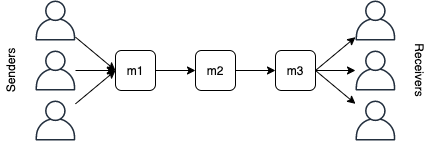
\includegraphics[width=\textwidth]{figures/topologies/cascade.png}
        \caption{Cascade}
        \label{fig:cascade}
    \end{subfigure}
    \hfill
    \begin{subfigure}[b]{0.45\textwidth}
        \centering
        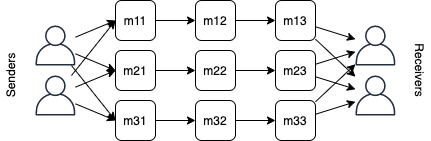
\includegraphics[width=\textwidth]{figures/topologies/multi-cascade.png}
        \caption{Multi-Cascade}
        \label{fig:multi-cascade}
    \end{subfigure}
    \hfill
    \begin{subfigure}[b]{0.45\textwidth}
        \centering
        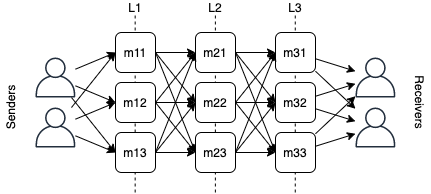
\includegraphics[width=\textwidth]{figures/topologies/stratified.png}
        \caption{Stratified}
        \label{fig:stratified}
    \end{subfigure}
    \hfill
    \begin{subfigure}[b]{0.45\textwidth}
        \centering
        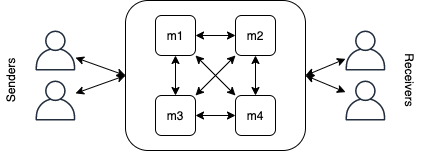
\includegraphics[width=\textwidth]{figures/topologies/mesh.png}
        \caption{Mesh}
        \label{fig:mesh}
    \end{subfigure}
       \caption{Mixnets Topologies}
       \label{fig:mixnets-topologies}
\end{figure}

\section{Mixing Techniques}

\begin{itemize}
   \item \textbf{Time-Based:} The time-based mixing technique aims to collect
   incoming messages and permute and forward them every t seconds, where t is a
   system-defined variable. Figure ... illustrates how time-based Mixes work.
   The advantage of this mixing technique is that we can control the message
   transfer delay. Nevertheless, the downside is that we do not get to govern
   how many messages we mix. This is because a different number of messages
   might be received in separate rounds. As a result, the number of messages
   shuffled each time is not the same; therefore, the anonymity set can
   sometimes be large while sometimes smaller. A small set of messages infers
   reduced anonymity. To keep anonymity above a baseline, we must incorporate
   complementary cover traffic, which comes with an extra computational expense.
   \item \textbf{Threshold-Based:} Similar to time-based mixes, a threshold Mix buffers
   messages into a queue until a predefined threshold is reached. Then we
   shuffle and forward messages to the next hop[]. In contrast with timed Mixes,
   threshold Mixes allow us to control the anonymity set of messages being
   processed. Nonetheless, this technique has some disadvantages as well.
   Primarily, the problem arises when the network does not have much traffic and
   the receiving buffer does not reach its limit shortly. As a result, message
   delivery will be delayed significantly, which is not ideal for the user
   experience. The solution to this problem is to integrate cover traffic in
   order to fill a Mix with messages more frequently. As mentioned before, this
   comes with a computational overhead.
   \item \textbf{Pool-Mix:} This hybrid mixing technique[25] derives features from timed,
   and threshold mixing approaches. In more detail, If a threshold is reached,
   we release a fraction of the messages every t seconds. The bright side of
   this realisation is that a message leaving the Mix can be either a new
   message which just entered the pool or an old one which was not picked during
   the last emission. There is no way of knowing which one was picked. As a
   result, anonymity is improved. At the same time, one could assume this
   feature is a bug. In other words, a message can stack in the pool for quite
   some time before arriving at its destination. We can observe that this yields
   unexpected delays. Besides that, a pool Mix requires many messages to work
   optimally. Therefore, as mentioned before, this solution might need to
   include cover traffic to increase the network's capacity.
   \item \textbf{Continues:} This mixing technique depends on a delay given by the
   message sender[26]. The advantage of this approach is that messages are not
   shuffled together, and therefore, there is no statistical inference. Each
   message is treated individually, and the dispatch timestamp is not affected
   by the arrival of any other message.
\end{itemize}

\section{Measuring Anonymity}

As many scientists stated in the past, "Entropy is the natural order of the
universe", meaning natural chaos. One way to measure anonymity in Mixnets is
entropy. In other words, we are trying to measure the chaos between message
transmissions. To do so, we use the Shannon entropy formula (the result is in
bits). Equation (2.1) describes that formula. High entropy values imply better
anonymity than lower values. There is no way of identifying acceptable entropy
levels since this depends on the network size and adversary capabilities. In the
following formula, we denote as $p(x)$ the probability that an attacker can
assign to a user being the message sender. For instance, if we have an anonymity
set of 1000 indistinguishable messages within a Mix buffer, we have 9.96 bits of
entropy ($Entropy = -\sum_{i = 1}^{1000}p(\frac{1}{1000}) \log_2p(\frac{1}{1000}) = 9.96 bits$). 

\begin{equation}
    \label{eq:entropy}
    H(X) = -\sum_{x \in X} p(x) \log_2p(x)     
\end{equation}

\begin{figure}[h!]
   \centering
   \begin{subfigure}[b]{0.45\textwidth}
       \centering
       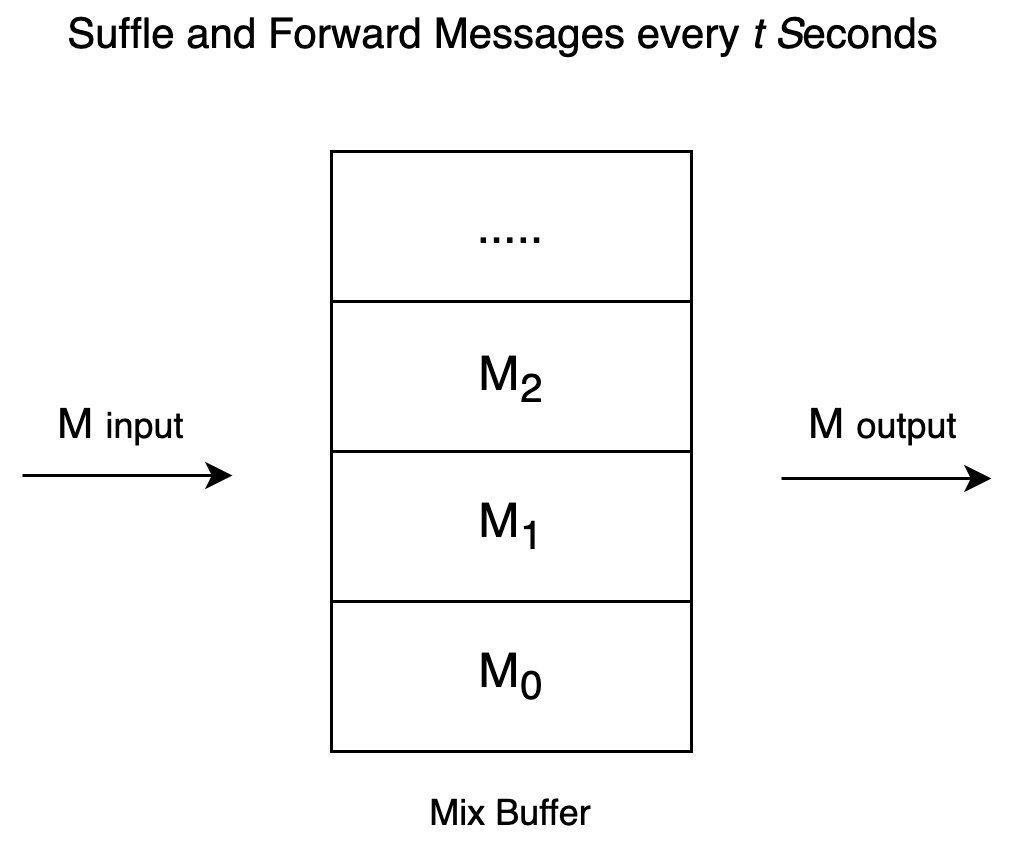
\includegraphics[width=\textwidth]{figures/mixing_techniques/timed.png}
       \caption{Timed Mix}
       \label{fig:Timed Mix}
   \end{subfigure}
   \hfill
   \begin{subfigure}[b]{0.45\textwidth}
       \centering
       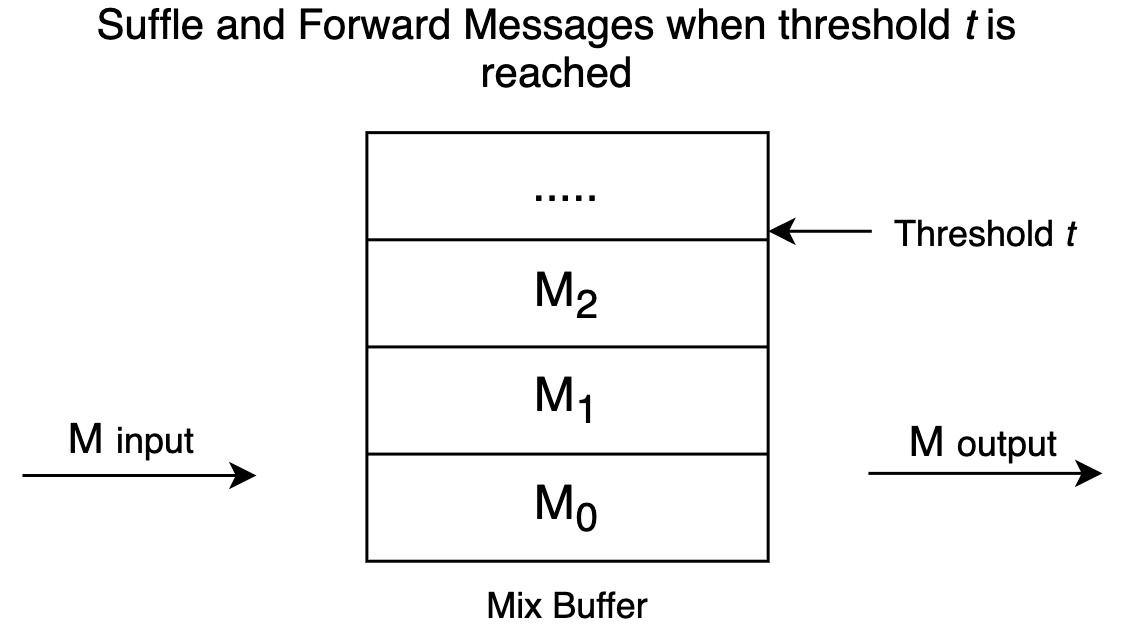
\includegraphics[width=\textwidth]{figures/mixing_techniques/threshold.png}
       \caption{Threshold Mix}
       \label{fig:Threshold Mix}
   \end{subfigure}
   \hfill
   \begin{subfigure}[b]{0.45\textwidth}
       \centering
       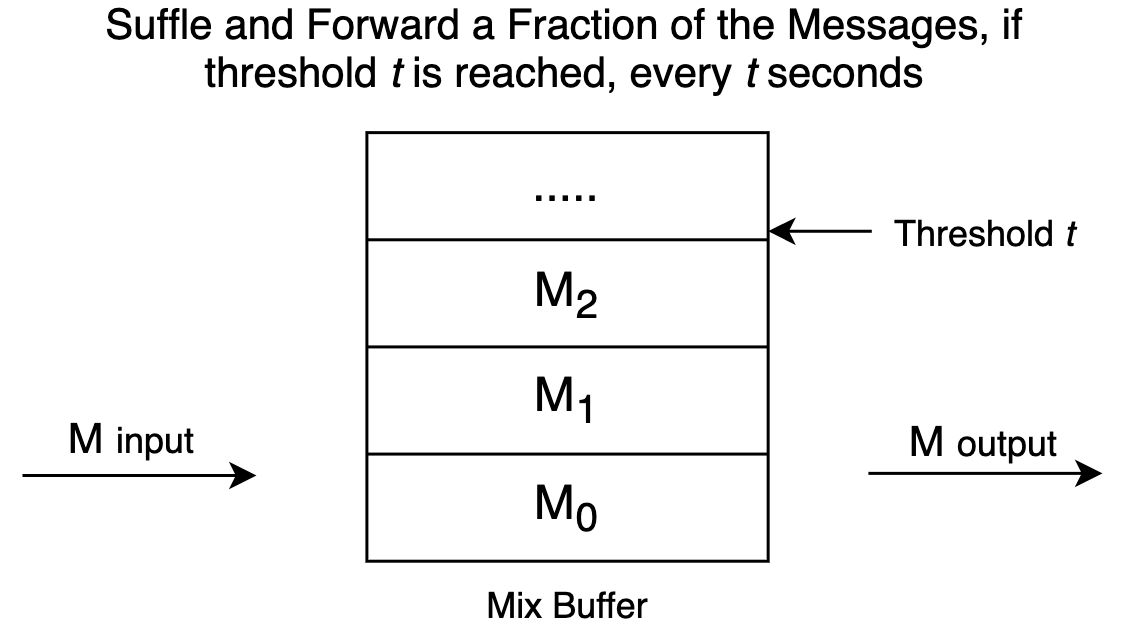
\includegraphics[width=\textwidth]{figures/mixing_techniques/pool.png}
       \caption{Pool Mix}
       \label{fig:Pool Mix}
   \end{subfigure}
   \hfill
   \begin{subfigure}[b]{0.45\textwidth}
       \centering
       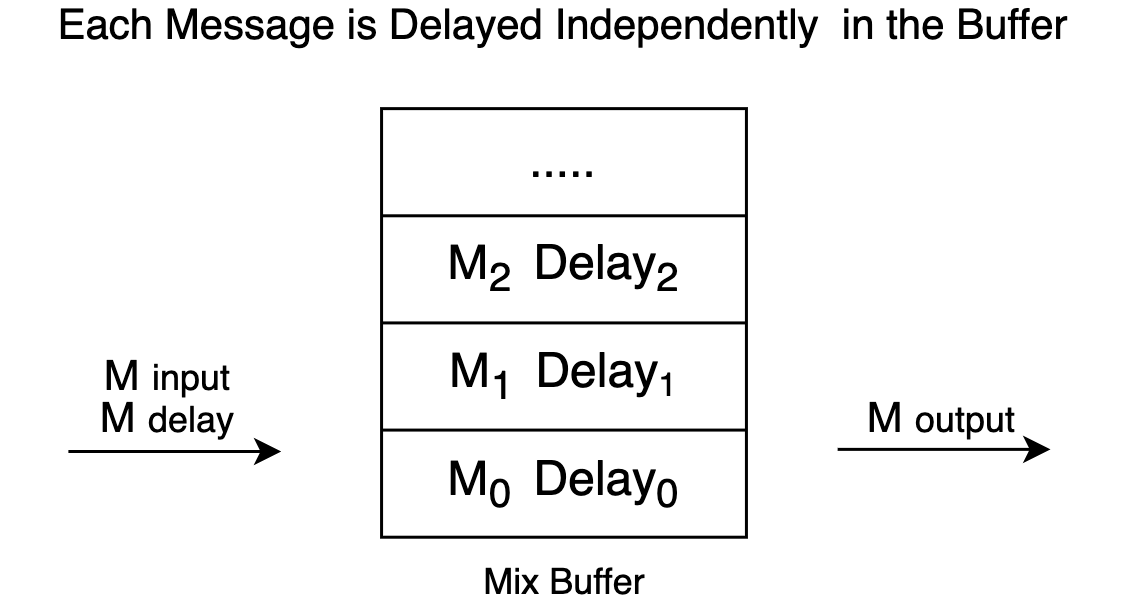
\includegraphics[width=\textwidth]{figures/mixing_techniques/continues.png}
       \caption{Continues Mix}
       \label{fig:Continues Mix}
   \end{subfigure}
      \caption{Mixnets Mixing Techniques}
      \label{fig:mixnets-mixing-techniques}
\end{figure}

\chapter{A Deep Dive Into The Simulators}

This chapter describes MiXiM and Simulator, criticising both projects
qualitatively and quantitatively. Next, we provide information about the
simulators' realisation, development decisions, execution workflow and supported
features. We also conduct a baseline experiment, measuring their needs for
computational resources. Finally, we aggregate this information on a competitive
grid to decide which software is potentially the best to adopt for future
research and development. 

\section{Simulator}
Piotrowska's work[] focuses on creating a simulator for evaluating the
anonymity, latency, bandwidth overhead and scalability of Mix Networks over
different design configurations. Her study mainly used the Simulator to compare
existing projects - Elixxir, HOPR and Nym - deployed on Mix Network
infrastructure with different layouts.

The developed software realises many features that capture real-world use cases
of Mix Networks, but it is not limited to it. Even though the simulator can
handle peer-to-peer (p2p) network simulations, we are not interested in such
network formations within the context of this project. Next, we will look deeper
into the Simulator's intrinsics, reporting on its core functionality, available
features and input parameters. Additionally, we will run the simulator against a
baseline configuration file using profiling tools[] and capture useful
information about the simulation execution. This type of information will
subsequently enable us to comment on simulation bottlenecks.

After analysing Piotrowska's simulator, we understood the code intrinsics and
captured its approach when simulating a network. The project is well-designed,
with the main simulation entities abstracted into classes. In particular, there
are abstractions for the following entities: (a) Network, (b) Mix Node, (c) Client,
(d) Message and (e) Packet. Even though it appears to exist a provision for
splitting messages into packages, it seems that this part of the code is
incomplete, and consequently, all messages are of one packet size.

Furthermore, this simulator allows users to run experiments given many options.
In more detail, there is support for many topologies, such as (a) Cascade, (b)
Multi-Cascade, (c) Stratified and (d) P2P. Besides, there is an option for two
mixing techniques (a) batch and reorder - threshold - and (b) poisson mixing
-continues. The current implementation has default-enabled cover traffic
generation for both clients and Mixes. Finally, the Simulator outputs the
anonymity metrics of (a) entropy and (b) unlinkability.

\subsection{Execution Workflow}

The workflow of executing a standard simulation scenario is as follows:

\begin{enumerate}
    \item Read user-generated configuration file.
    \item Initialize global/environment variables.
    \item Initialize Loggers.
    \item Create and initialize a Network object comprising a set of Clients and Mix Nodes.
    \item From the Clients' set, select two message senders and one recipient randomly.
    \item All clients begin generating cover traffic, while the initially
    elected senders will also generate real traffic. The message routing is
    selected randomly on every packet hop.
    \item The above process is simulated for three phases, burnin, execution,
    and cool down. During the burnin step, clients and Mixes generate only cover
    traffic, and no logging is performed. On the other hand, logging is enabled
    during the execution stage. During that phase, clients and Mixes send both
    real and cover traffic. We log entropy for every real message on every hop.
    Finally, we stop sending real messages during the cool-down phase while we
    continue sending dummy messages.
    \item Ultimately, the Simulator presents results to the user after
    inspecting the execution logs.
\end{enumerate}

\subsection{Input Parameters and Configuration File}

To begin with, the Simulator takes as input some command-line arguments defining
the simulation mode and necessary directories, where we can find the
configurations file, and directories where the output results will be dumped.
There follows a list of the accepted command-line arguments and their
description:

\begin{itemize}
    \item[] \texttt{-mode} \textbf{(required)} \textit{(string)}: This describes
    the mode in which we run the simulator. The accepted modes are \emph{test},
    \emph{test\_diff}, \emph{transcript}, \emph{synthetic traces}, and
    \emph{anon}; however, only the \emph{test} mode is entirely realised. We have no
    clue about the functionality or purpose of the other modes.
    \item[] \texttt{-exp\_dir} \textbf{(required)} \textit{(string)}: This argument
    declares the directory's path, where the Simulator will dump any experiment
    logging files.
    \item[] \texttt{-config\_file} \textbf{(required)} \textit{(string)}: This is
    the path to the configuration file, describing the simulation settings.
 \end{itemize}

The following command-line arguments are declared but never actually used in the
Simulator. We assume that a future continuation of this project will frame their
purpose. These arguments are \texttt{-test}, \texttt{-datadir}, \texttt{-hour},
\texttt{-12hour}, \texttt{-minute}, \texttt{-day}.

Moving to the configuration file, we can observe nine sections describing
different simulation aspects. We present a sample configuration file in Figure
...

\begin{itemize}
    \item \textbf{Section 1} - \emph{Experiment Id}: In this section, we provide
    a simple label to help keep different simulations in order.
    \item \textbf{Section 2} - \emph{Logging}: This section allows us to enable
    or disable logging. The attribute \texttt{dir} extends the logging directory path
    specified in the command-line arguments. The attributes \texttt{client\_log}
    and \texttt{mix\_log} shown in the configurations sample are never used
    throughout the simulation.
    \item \textbf{Section 3} - \emph{Simulation Phases}:  This section is
    related to simulation phases - burnin, execution and cool down. Mainly we
    can define the duration of each stage.
    \item \textbf{Section 4} - \emph{Network Topologies}:  This part of the file
    describes the supported network topologies of the simulator - Cascade,
    Stratified, Multi-Cascade and P2P - and their properties, such as the number
    of layers and layer size for stratified topologies or length and wideness
    for Cascade/Multi-Cascade topologies.
    \item \textbf{Section 5} - \emph{Packets}: This section defines the packet
    size (feature not realised).
    \item \textbf{Section 6} - \emph{Messages}: This section defines the message
    size (feature not realised, all messages are of length one packet).
    \item \textbf{Section 7} - \emph{Mixing Configurations}: Here, we can find
    Mixes settings like the average delay before sending a packet (continues
    mixing) and the batching of messages according to specific batch size
    (threshold mixing). 
    \item \textbf{Section 8} - \emph{Clients Information}: Here, we can specify
    information about clients, such as the number of participating clients, how
    often the client adds a real message to the send buffer, the send rate, and
    if the client is generating cover traffic, and if so, at what rate. It is
    important to note that the attributes \texttt{rate\_ack}, \texttt{ACK},
    \texttt{retransmit}, \texttt{dummies\_acks}, and
    \texttt{max\_retransmissions} are never used. 
    \item \textbf{Section 9} - \emph{miscellaneous}: This section keeps
    information denoting the length of a message-id and the number of total real
    messages we want to send during the simulation.
\end{itemize}

\subsection{Baseline Simulation and Profiling Measurements}

In our endeavour to assess Simulator, we run a series of experiments to identify
its performance and quality of results. In particular, the baseline simulation
examines the Simulator's behaviour in terms of space, memory, time complexity,
and the network's entropy. We run the same experiment for the three established
topologies - Cascade(10 Mixes), Multi-Cascade (3x10 Mixes) and Stratified (3x10
Mixes) - while increasing the simulation duration from 100 to 10000 time ticks.
We also configured the mixing technique to Poisson (i.e. Continues), the number
of clients to 100, and the number of target\_send\_messages to 1000. 

Our anticipation regarding memory usage is that all experiments will deliver the
same results for all topologies except Cascade. We establish our assumption on
the fact that a single Cascade topology has fewer Mixes than the other
topologies described earlier. However, according to Figure..., our hypothesis is
false since the Simulator uses the same amount of memory - roughly 247 megabytes
- in all experiments. In a later chapter, we will see that
memory usage solely depends on the number of users we are simulating.

In regards to space complexity, we expect to have differences among topologies.
Specifically, a Cascade Mixnet needs to route traffic through a chain of
nodes. The network's capacity aligns with a single mix's capacity. Therefore,
every time we dump each Mix's logs, we observe log lines to repeat because
messages stall there for a long time. A Multi-Cascade Mixnet performs better
since there are parallel chains of Mixes. The Stratified topology should be the
best since messages continually move from one Mix to another and do not repeat
in the log files so many times. Indeed, our hypothesis is accurate, and we can
notice that in Figure ...

Execution time should follow the same pattern as space complexity, given the
same reason concerning the nature of each topology, as noted before. We can
observe in Figure ... that this is mostly true, except for the Simulation
duration of 1000 time ticks. This negligible time offset on Figure ...  can be
caused by other processes running on our workstation at that moment.

Further, we need to check if Piotrowska's simulator reasonably captures the
notion of entropy for each topology. According to our measurements in Figure
..., Simulator reports higher entropy for Cascade topology. There follows Multi
Cascade and Stratified. These results are acceptable since aggregating more
messages on each hop increases Mix's anonymity set, so entropy is higher.

\begin{figure}[h!]
    \centering
    \begin{subfigure}[b]{0.45\textwidth}
        \centering
        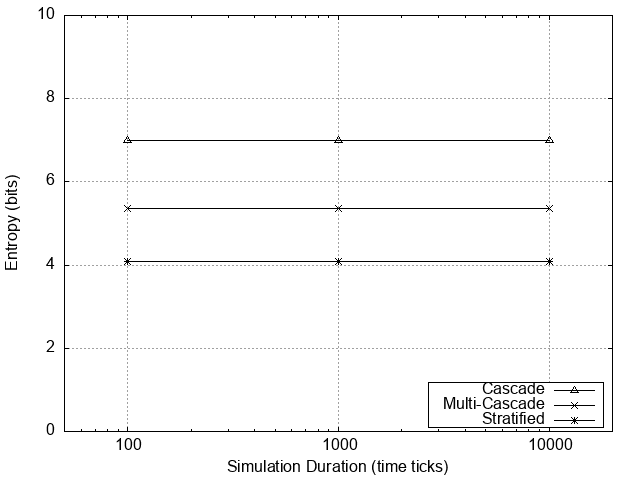
\includegraphics[width=\textwidth]{figures/baseline_simulation/simulator/baseline_simulator_entropy.png}
        \caption{Entropy}
        \label{fig:baseline-entropy}
    \end{subfigure}
    \hfill
    \begin{subfigure}[b]{0.45\textwidth}
        \centering
        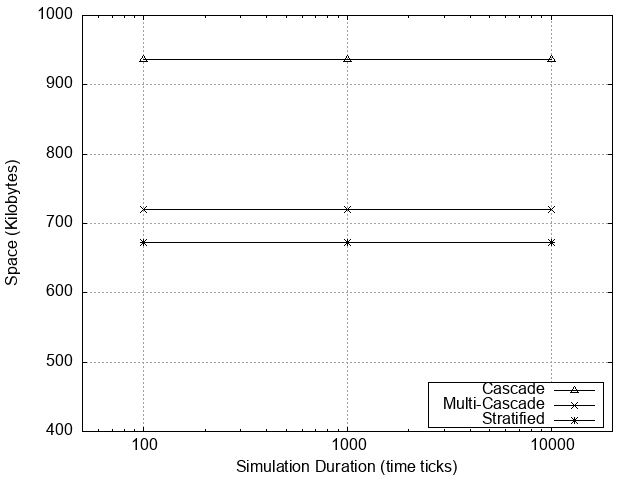
\includegraphics[width=\textwidth]{figures/baseline_simulation/simulator/baseline_simulator_space.png}
        \caption{Space}
        \label{fig:baseline-space}
    \end{subfigure}
    \hfill
    \begin{subfigure}[b]{0.45\textwidth}
        \centering
        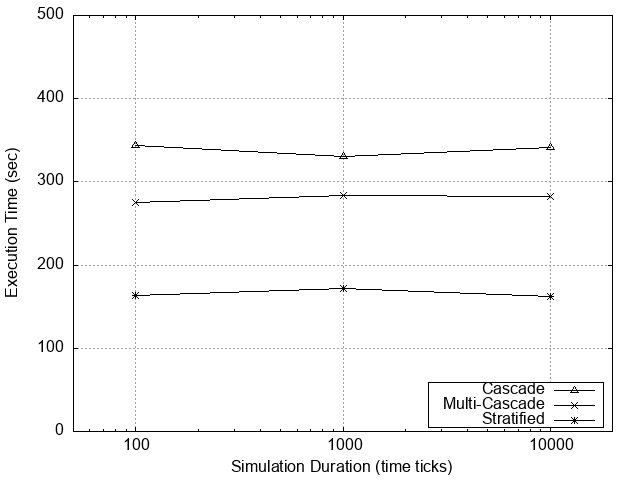
\includegraphics[width=\textwidth]{figures/baseline_simulation/simulator/baseline_simulator_time.png}
        \caption{Execution Time}
        \label{fig:baseline-time}
    \end{subfigure}
    \hfill
    \begin{subfigure}[b]{0.45\textwidth}
        \centering
        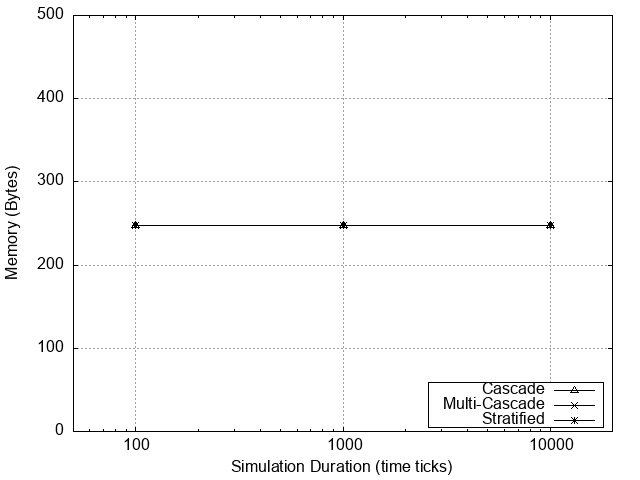
\includegraphics[width=\textwidth]{figures/baseline_simulation/simulator/baseline_simulator_mem.png}
        \caption{Memory}
        \label{fig:baseline-mem}
    \end{subfigure}
       \caption{Simulator Baseline Experiments}
       \label{fig:baseline-simulation}
 \end{figure}
 

Finally, we run Piotrowska's project using a \emph{cProfiler}[] to get visual
information and statistics about its execution tree (sequence of functions
called). We get a detailed representation of the execution tree in Figure. We
also analyze the project using \emph{SonarQube} to get information about the
quality of the code. In the first place, \emph{cProfiler} reveals that 59.75\%
of the CPU usage was for processing packets, while the heaviest task running
under the \emph{packet processing} branch was \emph{entropy update}. Entropy
update took 38.76\% of the total CPU usage, indicating a possible bottleneck to
the whole execution. Regarding \emph{SonarQube} results, we find out that 2.7\%
of the code is duplicated, and there are 57 \emph{code smells}, 2 \emph{bugs}
and 5 \emph{security issues} of no great importance.

\section{MiXiM}

Guirat et al. carried out a similar attempt to develop an event-driven Mix
Network simulator. In particular, Guirat et al., in their study[], present
MiXiM, a simulation framework that helps academics and industry professionals
assess design options and tradeoffs among different Mix Networks. Next, we will
delve into the simulator implementation, reporting on its functionality,
available features and input parameters. Besides that, we aim to run the
simulator against a baseline scenario, reporting on its outputs and execution
statistics. This information will help us decide if MiXiM is a well-built and
feature-proof tool that brings out the most.

After analyzing MiXiM, we understood the code intrinsics and captured its
approach when simulating a network. Likewise, Piotrowska's work is well-designed
and abstracted into similar entities: a)Simulation, b) Network, c) Mix
Node(Poisson Mix, Pool, Timed Mix), d) Client, e) Relay(abstraction of an
attacker) and f) Message.

Furthermore, the simulator allows users to run experiments given various
configurations. In more detail, there is support for many topologies, such as
(1) cascade, (2) multi-cascade, and (3) stratified. Additionally, there is an
option for three mixing techniques (1) Timed mixing and (2) Poisson mixing and
(3) Threshold Mixing. Besides that, the users can enable dummy traffic
generation, giving a specific generation rate. Another outstanding feature is
the introduction of corrupted mix nodes during the simulation. Finally, the
Simulator outputs the anonymity metric of entropy.

\subsection{Execution Workflow}

The workflow of executing a standard simulation scenario is as follows:

\begin{enumerate}
    \item Read user-generated configuration file.
    \item Create and initialize a simulation object passing all the input
    parameters found in step 1.
    \item Call the run function of the simulation object.
    \item Create and initialize a Network object comprising a set of Clients and
    Mix Nodes, including possible corrupted nodes. Connect nodes with their
    neighbours.
    \item Then all clients begin generating traffic according to the given $\lambda$
    generation variable. In the meantime, dummy traffic is generated as well.
    \item The simulation is executed in a single phase lasting for several time
    ticks declared in the configuration file. During each message transmission
    from one node to another, entropy is updated.
    \item Ultimately, MiXiM presents the average results to the user after
    inspecting the execution logs.
\end{enumerate}

\subsection{Input Parameters and Configuration File}

MiXiM, compared to Simulator, does not take any command-line arguments. We only
observe a single configuration file with six different sections. We present a
sample configuration file in Figure 2. Following, we provide a thorough
description of the aforementioned file.

In the first place, we can see under the DEFAULT section the number of clients
sending and receiving messages in a network and a parameter called lambda\_c
representing the rate of generating messages per time tick. Next, under the
TOPOLOGY section, we can see different settings for all three supported
topologies - Stratified, Cascade and Free Route. We can use the parameter
fully\_connected to decide if we want to have mixes fully connected. The user can
also define the routing strategy by choosing between the source or hop by hop.
Other parameters in this section include E2E, the minimum end-to-end
transmission delay, and n\_layers, l\_mixes\_per\_layer and n\_cascades, which
describe the Cascade or stratified topology number of layers and the
corresponding number of mixes that each layer hosts. Subsequently, we observe a
section explaining the available mixing techniques. We have the mix\_type, which
can be Poisson, Time, or Pool and mu, which is the delay on each mix node. For
each of the aforementioned mixing techniques, the variables timeout, threshold,
and flush\_percent, match each case accordingly. The following section refers to
dummy data generation. The user can set the variables client\_dummies to enable
or disable dummy, rate\_client\_dummies to control the dummy data generation,
link\_based\_dummies to send dummies dropped on the next hop, multiple\_hop\_dummies
to send dummies that last for many hops, and rate\_mix\_dummies to generate dummy
messages on the Mix. The subsequent section, NODE\_SELECTION, is not required
during the simulation and might have been left there from older software
versions. Finally, we got the THREAT\_MODEL section, where we define the number
of corrupted nodes and if we can uniformly distribute them across the network
layers.

\subsection{Baseline Simulation and Profiling Measurements}

Section 3.1.3 described our attempt to evaluate the Simulator according to a
baseline scenario. We make the same assumptions for MiXiM, running the same
experiments. Unfortunately, our expectations did not match the results since we
could not reproduce every simulation.

Mainly, we managed to simulate Stratified topologies for 100 and 1000 time
ticks. Attempting to run experiments for Cascade and Multi-Cascade network
arrangements failed due to run-time errors. Simulating a Stratified topology for
10000 time ticks also resulted in a crash. We were hesitant about the failure
causes, so we decided to probe the software code-base to uncover potential
issues.

Indeed, skimming the source code, we managed to spot four bugs we present in the following list. 

\begin{enumerate}
    \item The parsing section of the code accepts as valid topologies "cascade",
    "multi-cascade", and "stratified". Nevertheless, this is not the case for
    some files - Network.py, Simulation.py and Client.py - where the code
    expects a topology called "XDR".
    \item The variable n\_cascade, which describes the number of parallel
    Cascades in Network.py, is hard coded. Hence, the simulation is not assuming
    the user's configuration.
    \item In file Simulation.py, a variable is declared as otherClient, while
    the software developer used the name other\_client when initialising the
    variable. Consequently, the initialisation is meaningless, and otherClient
    has no value.
    \item The initial parsing of boolean parameters from the configuration file
    is incorrect since the code used is a Python2 command which, when using
    Python3, always returns True. Therefore all boolean parameters in the
    configuration file are True, no matter their actual value.
\end{enumerate}

The purpose of this project is not to fix someone else's work but asses it.
Consequently, we did not proceed with further code reviews or repairs.

In regards to the conducted experiments, we can observe the results in Figure.
We cannot deduce valuable insights from these graphs since, as mentioned
earlier, we failed to fulfil all of them. Surprisingly, the execution time and
space used to dump log files increase linearly for different simulation
time-frames. According to our previous code analysis, this is expected since
clients in MiXiM generate messages based on the $\lambda$ rate. Therefore, the
longer the simulation, the more messages are generated. Hence, more processing
time and storage space are required. Instead, the Simulator simulates only the
number of specified target messages regardless of the duration. Furthermore, it
is notable that in terms of memory usage, MiXiM is sufficient, requiring only
21.4 megabytes of RAM. 

\begin{figure}[h!]
    \centering
    \begin{subfigure}[b]{0.45\textwidth}
        \centering
        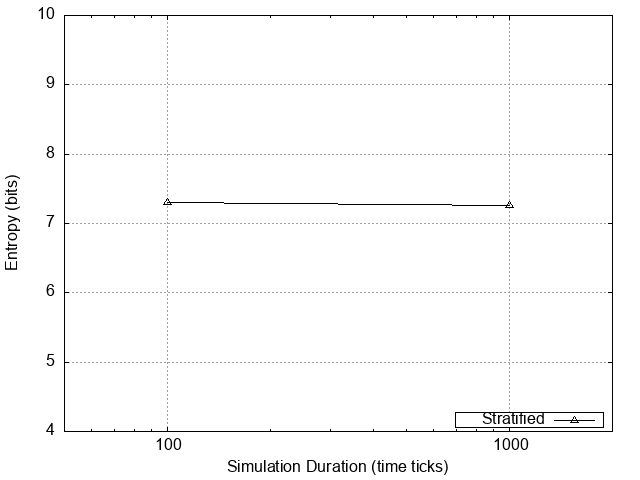
\includegraphics[width=\textwidth]{figures/baseline_simulation/mixim/baseline_mixim_entropy.png}
        \caption{Entropy}
        \label{fig:baseline-mixim-entropy}
    \end{subfigure}
    \hfill
    \begin{subfigure}[b]{0.45\textwidth}
        \centering
        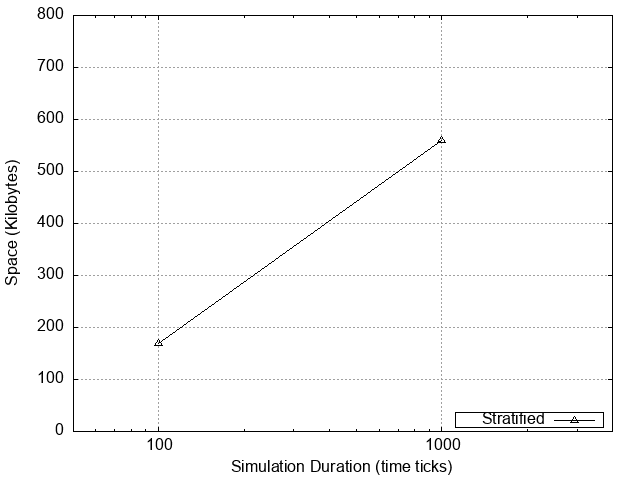
\includegraphics[width=\textwidth]{figures/baseline_simulation/mixim/baseline_mixim_space.png}
        \caption{Space}
        \label{fig:baseline-mixim-space}
    \end{subfigure}
    \hfill
    \begin{subfigure}[b]{0.45\textwidth}
        \centering
        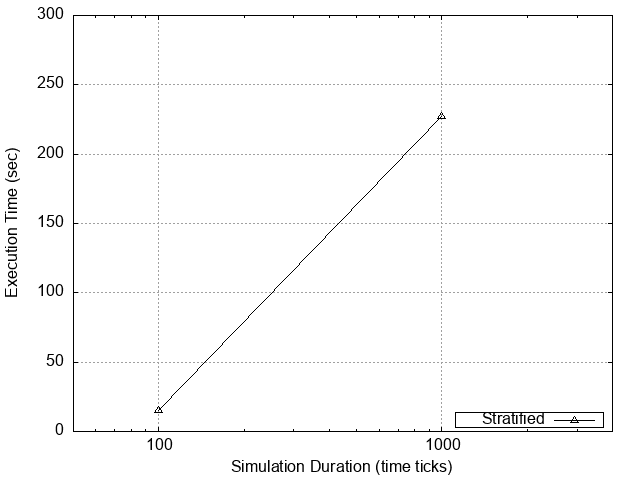
\includegraphics[width=\textwidth]{figures/baseline_simulation/mixim/baseline_mixim_time.png}
        \caption{Execution Time}
        \label{fig:baseline-mixim-time}
    \end{subfigure}
    \hfill
    \begin{subfigure}[b]{0.45\textwidth}
        \centering
        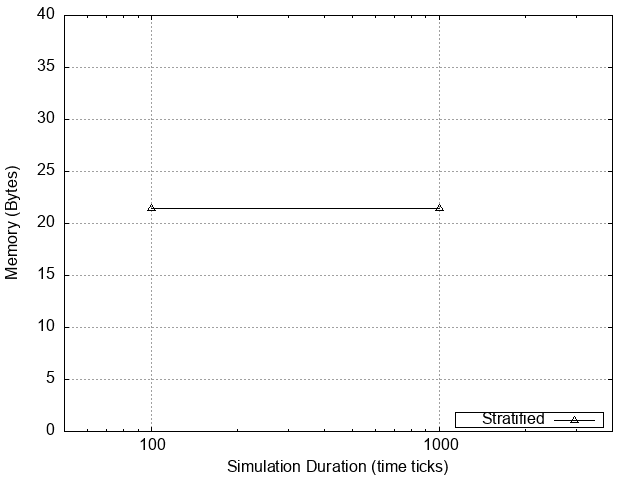
\includegraphics[width=\textwidth]{figures/baseline_simulation/mixim/baseline_mixim_mem.png}
        \caption{Memory}
        \label{fig:baseline-mixim-mem}
    \end{subfigure}
       \caption{MiXiM Baseline Experiments}
       \label{fig:baseline-mixim-simulation}
 \end{figure}


\section{Compasisson Framework}

To bring conclusiveness to our simulator analysis, we present in this section a
comparison framework. Our ultimate goal is to find out which simulator is better
to adopt for further development in the future. A comprehensive comparison
framework needs to evaluate multiple factors. Therefore we assumed the following
KPIs (key performance indicators) (a) Topologies, (b) Mixing Techniques, (c)
Routing Methods for Stratified topology, (d) Cover Traffic, (e) Corrupt Relays,
and (f) SonarQube Code analysis insights.

\begin{table}[h!]
    \begin{center}
        \begin{tabular}{||c|l|c|c||}
            \hline
                                                                &                               & Simulator   & MiXiM         \\ \hline
            \multirow{5}{*}{Topologies}                         & Cascade                       & \ding{51}   & \ding{51}         \\ \cline{2-4} 
                                                                & Multi-Cascade                 & \ding{51}        & \ding{51}          \\ \cline{2-4} 
                                                                & Stratified - Fully Connected  & \ding{51}        & \ding{51}          \\ \cline{2-4} 
                                                                & Stratified - Semi Connected   &               & \ding{51}          \\ \cline{2-4} 
                                                                & P2P                           & \ding{51}       &                  \\ \hline \hline
            \multirow{4}{*}{Mixing Techniques}                  & Timed                         &                & \ding{51}          \\ \cline{2-4} 
                                                                & Threshold                     & \ding{51}       & \ding{51}          \\ \cline{2-4} 
                                                                & Pool                          &                & \ding{51}          \\ \cline{2-4} 
                                                                & Continues                     & \ding{51}      & \ding{51}          \\ \hline \hline
            Routing                                             & Random Choice                 & \ding{51}      & \ding{51}         \\ \hline \hline
            \multirow{3}{*}{Cover Traffic}                      & On Client                     & \ding{51}       & \ding{51}         \\ \cline{2-4} 
                                                                & On Mix                        & \ding{51}       & \ding{51}         \\ \cline{2-4} 
                                                                & Multi-hop Dummies             &                & \ding{51}         \\ \hline \hline
            Relays                                              & Corrupt Mixes                 &                & \ding{51}          \\ \hline \hline
            \multirow{7}{*}{Code Analysis}                      & Code Readability              & 4/5            & 2/5              \\ \cline{2-4}
                                                                & Object Abstraction            & 5/5             & 5/5               \\ \cline{2-4}
                                                                & Code Smells                   & 57            & 81                \\ \cline{2-4}
                                                                & Bugs                          & 2             & 4                  \\ \cline{2-4}
                                                                & Security Issues               & 5              & 10                \\ \cline{2-4}
                                                                & Duplicate Code                & 2.7\%        & 0\%               \\ \cline{2-4}
                                                                & Runtime Crashes               &                  & \ding{51}            \\ \hline \hline
            \end{tabular}
    \end{center}
    
    \caption{Simulators Comparisson Table}
    \label{tab:comparisson-table}
    \end{table}

Table ... illustrates how MiXiM and Simulator compare in each aspect. We notice
that MiXiM realises 13 features, while Simulator has only 9. Nonetheless, it is
essential to prompt that most of MiXiM's features are not working (look section
...) and simulations crash on runtime. Also, both software achieves high scores
in object abstraction, while code readability for MiXiM seems to be poor.
Further, MiXiM has 81 code smells compared to Simulator, which has 57. Moreover,
MiXiM has double the bugs and security issues compared to Simulator, which has 2
and 5, respectively. Finally, both projects have negligible amounts of code
duplication.

Eventually, we decided that the best simulator so far is Piotrawskas Simulator.
We justify our decision mainly based on the usability aspect. Even though MiXiM
advertises a large set of features, it fails to deliver a working code-base. We
are confident that Simulator is a well-designed software and can be improved so
in the future support more features. 

\chapter{Replication Study}

\section{Studying the Anonymity Trilemma with Discrete-event Mix Network Simulator}

\section{MiXiM: Design Decisions and Empirical Evaluation}

\chapter{Imbalanced Stratified Mix Networks Study}

\section{Dynamically Imbalanced Stratified Network}

\section{Statically Imbalanced Stratified Network}

\chapter{Conclusion}

\section{Final Reminder}

The body of your dissertation, before the references and any appendices,
\emph{must} finish by page~40. The introduction, after preliminary material,
should have started on page~1.

You may not change the dissertation format (e.g., reduce the font size, change
the margins, or reduce the line spacing from the default 1.5 spacing). Be
careful if you copy-paste packages into your document preamble from elsewhere.
Some \LaTeX{} packages, such as \texttt{fullpage} or \texttt{savetrees}, change
the margins of your document. Do not include them!

Over-length or incorrectly-formatted dissertations will not be accepted and you
would have to modify your dissertation and resubmit. You cannot assume we will
check your submission before the final deadline and if it requires resubmission
after the deadline to conform to the page and style requirements you will be
subject to the usual late penalties based on your final submission time.

\bibliographystyle{plain}
\bibliography{mybibfile}


% You may delete everything from \appendix up to \end{document} if you don't need it.
\appendix

\chapter{First appendix}

\section{First section}

Any appendices, including any required ethics information, should be included
after the references.

Markers do not have to consider appendices. Make sure that your contributions
are made clear in the main body of the dissertation (within the page limit).

\chapter{Participants' information sheet}

If you had human participants, include key information that they were given in
an appendix, and point to it from the ethics declaration.

\chapter{Participants' consent form}

If you had human participants, include information about how consent was
gathered in an appendix, and point to it from the ethics declaration.


\end{document}
